\chapter{Introduction} \label{chapter1}

\section{Motivation}
During the last several months entire Europe has faced a new migration crisis with over 6 million people fleeing Ukraine to the neighboring countries following the full-scale Russian military invasion. This became a true challenge for almost all European countries including Switzerland. For the first time in its history Switzerland has given refugees the right to obtain residency with minimal administrative effort (Status S, 2022). This created a situation when numerous public services (migration office, social services, etc.), NGOs, private organizations as well as local administration had to quickly react and coordinate their efforts.

Digitalization plays a crucial role in the orchestration of a situation with various stakeholders (refugees, administrative workers, volunteers, etc.) in a such critical moment and could possibly facilitate administrative processes at different levels. Nevertheless, currently the usage of the digital platforms is mostly limited to information exchange. For example, the website of the canton of Zurich (Figure~\ref{fig:1}) provides information for various stakeholders such as refugees, volunteers, local administrations, but no interaction between the actors is possible \citep{Ukraine-Hilfe}. At the same time a matching platform for accommodation search and proposal was rapidly developed by a private organization and has timely reacted in the crisis situation (Ukraine Campax, 2022). Moreover, due to the lack of German language knowledge official websites are to a large extent inaccessible to the refugees and this led to the intensive use of alternative digital platforms such as Facebook or Telegram groups.

\begin{figure*}[tbp]
\centering
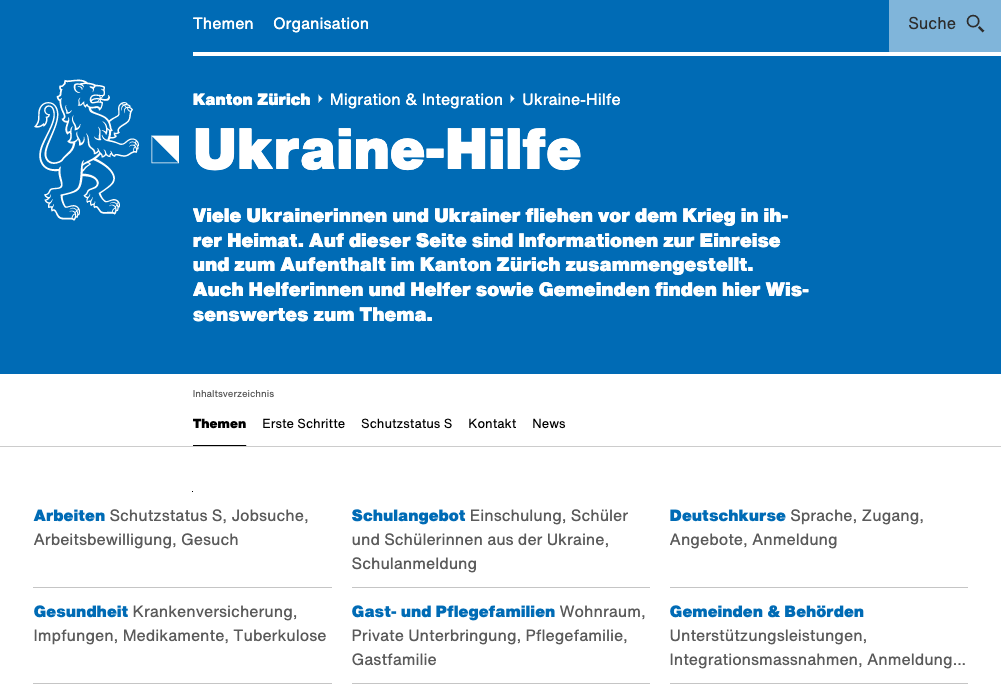
\includegraphics[width=8cm]{Figures/Ukraine_Hilfe.jpg}
\caption{Website of the Canton of Zurich.}
\label{fig:1}
\end{figure*}

In order for public administration to produce more efficient digital services that could handle such crisis situations an approach know as Government as a Platform (GaaP) could be adopted. The concept of GaaP implies the creation of an open platform for public sector where various actors within and outside public administration can introduce innovative ideas and together create better public services \citep{Reilly:2011}. GaaP promotes public sector efficiency, collaboration of stakeholders through openness and participation, and user-friendliness of public services \citep{Cordella2019, janssen2013lean}.

The proposed bachelor thesis will be prepared as part of the DIZH Rapid Action Call project “'Government as/is a platform': Orchestrating stakeholders in crisis situations through digital platforms in the canton of Zurich”. The given thesis will focus on the analysis and design of an architecture for a digital platform solution for the canton of Zurich based on a series of expert interviews with cantonal public administrations.

\section{Research Questions}

The following research questions will be addressed in this thesis:

RQ 1: What are the existing approaches and design principles for digital platforms available to administrate crisis situations such as Ukrainian crisis?

RQ 2: How does the public administration of the Canton of Zurich orchestrate the interaction of multiple actors involved in the Ukrainian crisis with the existing digital platforms?

RQ 3: How could the existing digital platforms of the Canton of Zurich be enhanced in order to react timely in a crisis situation such as the current refugee crisis?

\section{Thesis Outline}

The structure of this thesis will take the following form. 